\documentclass[border=10pt]{standalone}
\usepackage{tikz}
\usepackage{amsmath}
\usetikzlibrary{shapes.geometric, arrows.meta, positioning, calc, backgrounds, fit}

% 定义颜色
\definecolor{inputgreen}{RGB}{67, 160, 71}
\definecolor{sablue}{RGB}{30, 136, 229}
\definecolor{globalorange}{RGB}{251, 140, 0}
\definecolor{fcred}{RGB}{229, 57, 53}
\definecolor{softmaxcyan}{RGB}{0, 172, 193}
\definecolor{gtgreen}{RGB}{85, 139, 47}
\definecolor{lossred}{RGB}{211, 47, 47}
\definecolor{probpurple}{RGB}{171, 71, 188}
\definecolor{graybox}{RGB}{120, 144, 156}

% 定义3D块样式
\tikzset{
    block3d/.style={
        draw=black!70,
        line width=0.4pt,
        minimum height=#1,
        minimum width=0.6cm,
        fill=#1,
        inner sep=0pt,
    },
    sa/.style={
        draw=black!70,
        fill=sablue,
        minimum height=1.8cm,
        minimum width=0.7cm,
        rounded corners=2pt,
    },
    fc/.style={
        draw=black!70,
        fill=fcred,
        minimum height=1.2cm,
        minimum width=0.5cm,
        rounded corners=2pt,
    },
    opbox/.style={
        draw=black!70,
        fill=#1,
        minimum height=0.6cm,
        minimum width=1.2cm,
        rounded corners=3pt,
        font=\small\bfseries,
        text=white,
    },
    probbox/.style={
        draw=black!70,
        fill=#1,
        minimum height=0.8cm,
        minimum width=0.8cm,
        rounded corners=3pt,
        font=\normalsize\bfseries,
        text=white,
    },
    lossnode/.style={
        draw=lossred!80!black,
        fill=lossred,
        circle,
        minimum size=1.2cm,
        font=\small\bfseries,
        text=white,
        line width=1pt,
    },
    arrow/.style={
        ->,
        >=Stealth,
        line width=0.6pt,
        color=black!60,
    },
    redarrow/.style={
        ->,
        >=Stealth,
        line width=0.8pt,
        color=lossred,
    },
    label/.style={
        font=\scriptsize,
        text=black!70,
    },
    blocklabel/.style={
        font=\footnotesize\bfseries,
        text=white,
    },
}

\begin{document}
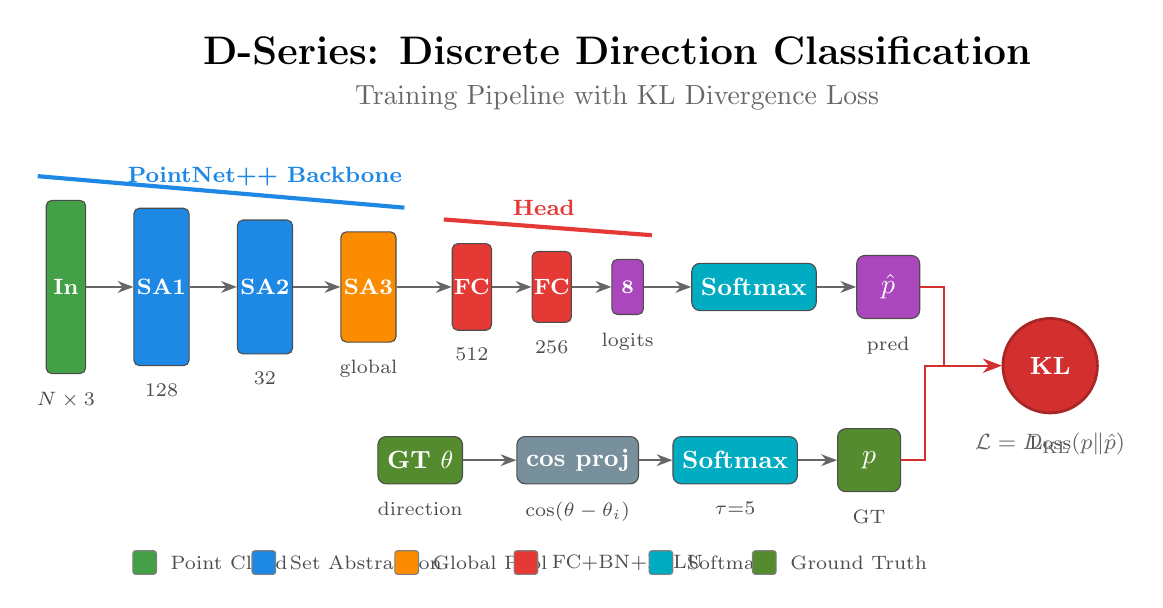
\begin{tikzpicture}[node distance=0.5cm]

% ===== 标题 =====
\node[font=\Large\bfseries] (title) at (7, 4) {D-Series: Discrete Direction Classification};
\node[font=\normalsize, text=black!60] at (7, 3.4) {Training Pipeline with KL Divergence Loss};

% ===== 主网络 =====
% Input
\node[draw=black!70, fill=inputgreen, minimum height=2.2cm, minimum width=0.5cm, rounded corners=2pt] (input) at (0, 1) {};
\node[blocklabel] at (input) {In};
\node[label, below=0.1cm of input] {$N\times3$};

% SA1
\node[sa, minimum height=2cm, right=0.6cm of input] (sa1) {};
\node[blocklabel] at (sa1) {SA1};
\node[label, below=0.1cm of sa1] {128};

% SA2
\node[sa, minimum height=1.7cm, right=0.6cm of sa1] (sa2) {};
\node[blocklabel] at (sa2) {SA2};
\node[label, below=0.1cm of sa2] {32};

% SA3
\node[draw=black!70, fill=globalorange, minimum height=1.4cm, minimum width=0.7cm, rounded corners=2pt, right=0.6cm of sa2] (sa3) {};
\node[blocklabel] at (sa3) {SA3};
\node[label, below=0.1cm of sa3] {global};

% FC1
\node[fc, minimum height=1.1cm, right=0.7cm of sa3] (fc1) {};
\node[blocklabel] at (fc1) {FC};
\node[label, below=0.1cm of fc1] {512};

% FC2
\node[fc, minimum height=0.9cm, right=0.5cm of fc1] (fc2) {};
\node[blocklabel] at (fc2) {FC};
\node[label, below=0.1cm of fc2] {256};

% Logits
\node[draw=black!70, fill=probpurple, minimum height=0.7cm, minimum width=0.4cm, rounded corners=2pt, right=0.5cm of fc2] (logits) {};
\node[blocklabel, font=\scriptsize\bfseries] at (logits) {8};
\node[label, below=0.1cm of logits] {logits};

% Softmax
\node[opbox=softmaxcyan, right=0.6cm of logits] (softmax) {Softmax};

% Pred probs
\node[probbox=probpurple, right=0.5cm of softmax] (predp) {$\hat{p}$};
\node[label, below=0.1cm of predp] {pred};

% 箭头 - 主网络
\draw[arrow] (input) -- (sa1);
\draw[arrow] (sa1) -- (sa2);
\draw[arrow] (sa2) -- (sa3);
\draw[arrow] (sa3) -- (fc1);
\draw[arrow] (fc1) -- (fc2);
\draw[arrow] (fc2) -- (logits);
\draw[arrow] (logits) -- (softmax);
\draw[arrow] (softmax) -- (predp);

% ===== GT分支 =====
% GT theta
\node[opbox=gtgreen, minimum width=1cm] (gttheta) at (4.5, -1.2) {GT $\theta$};
\node[label, below=0.1cm of gttheta] {direction};

% cos projection
\node[opbox=graybox] (cosproj) at (6.5, -1.2) {cos proj};
\node[label, below=0.1cm of cosproj] {$\cos(\theta-\theta_i)$};

% GT Softmax
\node[opbox=softmaxcyan] (gtsoftmax) at (8.5, -1.2) {Softmax};
\node[label, below=0.1cm of gtsoftmax] {$\tau$=5};

% GT probs
\node[probbox=gtgreen] (gtp) at (10.2, -1.2) {$p$};
\node[label, below=0.1cm of gtp] {GT};

% 箭头 - GT分支
\draw[arrow] (gttheta) -- (cosproj);
\draw[arrow] (cosproj) -- (gtsoftmax);
\draw[arrow] (gtsoftmax) -- (gtp);

% ===== KL Loss =====
\node[lossnode] (loss) at (12.5, 0) {KL};
\node[label, below=0.15cm of loss, font=\scriptsize] {Loss};
\node[font=\footnotesize, text=black!60] at (12.5, -1) {$\mathcal{L}=D_{\text{KL}}(p\|\hat{p})$};

% 箭头到Loss
\draw[redarrow] (predp.east) -- ++(0.3,0) |- (loss.west);
\draw[redarrow] (gtp.east) -- ++(0.3,0) |- (loss.west);

% ===== 模块标注 =====
\draw[sablue, line width=1.5pt] ($(input.north west)+(-0.1,0.3)$) -- ($(sa3.north east)+(0.1,0.3)$);
\node[font=\footnotesize\bfseries, text=sablue] at ($(sa2.north)+(0,0.55)$) {PointNet++ Backbone};

\draw[fcred, line width=1.5pt] ($(fc1.north west)+(-0.1,0.3)$) -- ($(logits.north east)+(0.1,0.3)$);
\node[font=\footnotesize\bfseries, text=fcred] at ($(fc2.north)+(-0.1,0.55)$) {Head};

% ===== 图例 =====
\node[draw=black!50, fill=inputgreen, minimum size=0.3cm, rounded corners=1pt] (leg1) at (1, -2.5) {};
\node[label, right=0.05cm of leg1, font=\scriptsize] {Point Cloud};

\node[draw=black!50, fill=sablue, minimum size=0.3cm, rounded corners=1pt, right=1.2cm of leg1] (leg2) {};
\node[label, right=0.05cm of leg2, font=\scriptsize] {Set Abstraction};

\node[draw=black!50, fill=globalorange, minimum size=0.3cm, rounded corners=1pt, right=1.5cm of leg2] (leg3) {};
\node[label, right=0.05cm of leg3, font=\scriptsize] {Global Pool};

\node[draw=black!50, fill=fcred, minimum size=0.3cm, rounded corners=1pt, right=1.2cm of leg3] (leg4) {};
\node[label, right=0.05cm of leg4, font=\scriptsize] {FC+BN+ReLU};

\node[draw=black!50, fill=softmaxcyan, minimum size=0.3cm, rounded corners=1pt, right=1.4cm of leg4] (leg5) {};
\node[label, right=0.05cm of leg5, font=\scriptsize] {Softmax};

\node[draw=black!50, fill=gtgreen, minimum size=0.3cm, rounded corners=1pt, right=1cm of leg5] (leg6) {};
\node[label, right=0.05cm of leg6, font=\scriptsize] {Ground Truth};

\end{tikzpicture}
\end{document}
